% =============================================================================
% CS224R IPO + RLOO Milestone Report Template
% =============================================================================
% This template provides a suggested structure for your CS224R milestone report.
% Please ensure your report addresses all requirements for the IPO and RLOO components.
% =============================================================================

\documentclass{article}

\usepackage[preprint]{cs224r_2026}
\usepackage[utf8]{inputenc} % allow utf-8 input
\usepackage[T1]{fontenc}    % use 8-bit T1 fonts
\usepackage{hyperref}       % hyperlinks
\usepackage{url}            % simple URL typesetting
\usepackage{booktabs}       % professional-quality tables
\usepackage{amsfonts}       % blackboard math symbols
\usepackage{nicefrac}       % compact symbols for 1/2, etc.
\usepackage{microtype}      % microtypography
\usepackage{xcolor}         % colors
\usepackage{amsmath}
\usepackage{fancyhdr}       % for headers and footers
\usepackage{graphicx}   
\usepackage{float}
% for including figures
\usepackage{enumitem}       % for custom enumeration
\usepackage{listings}       % for formatting rollouts/code blocks

% Setup header
\pagestyle{fancy}
\fancyhf{} % clear all header and footer fields
\fancyhead[C]{CS224R IPO + RLOO Milestone Report}
\renewcommand{\headrulewidth}{0.4pt}

% Custom listing style for rollouts
\lstset{
  basicstyle=\small\ttfamily,
  breaklines=true,
  frame=single,
  backgroundcolor=\color{gray!5},
  rulecolor=\color{gray!30},
  columns=fullflexible,
  keepspaces=true,
  captionpos=b
}

% Custom title format for milestone document
\renewcommand{\maketitle}{
  \begin{center}
    {\bf \large CS224R Milestone: IPO + RLOO Alignment Report}\\
    \vspace{0.15cm}
    {\bf Project Title: Conjecturer-Prover Self-Play for Countdown Arithmetic Reasoning}\\
    \vspace{0.1cm}
    {\bf Team Members:} Nick Allen, Finn Staeblein\\
    \vspace{0.1cm}
    {\bf Emails:} nallen21@stanford.edu, finnst@stanford.edu
    \vspace{0.2cm}
  \end{center}
}

\begin{document}

\maketitle

\vspace{0.3cm}

\section{IPO Milestone Component}
\label{sec:ipo_milestone}

\subsection{Training and Evaluation Metrics}
We initialize the policy from our SFT checkpoint and run IPO for one epoch over
roughly 48{,}000 preference pairs, using a learning rate of $5\times10^{-6}$,
$\beta = 0.1$, and the AdamW optimizer. The reference model is the frozen SFT
checkpoint, evaluated under \texttt{no\_grad}.

For each preference pair we compute the difference of log-ratios
\[
h = \big(\log \pi_\theta(y_w \mid x) - \log \pi_{\text{ref}}(y_w \mid x)\big)
  - \big(\log \pi_\theta(y_l \mid x) - \log \pi_{\text{ref}}(y_l \mid x)\big),
\]
where $y_w$ is the chosen response and $y_l$ the rejected one, and each
log-probability is the sum of token log-probabilities over response tokens only
(prompt and padding positions are masked out). The IPO loss is a squared error
that pushes $h$ toward the target margin $1/(2\beta) = 5$:
\[
\mathcal{L}_{\text{IPO}} = \Big(h - \tfrac{1}{2\beta}\Big)^2 .
\]
We log the reward margin $(\beta h)$ averaged over the batch, and the reward
accuracy, the fraction of pairs for which the chosen log-ratio exceeds the
rejected log-ratio. Training was stable. The reward margin stayed positive
throughout and reward accuracy reached about $0.68$ on the train set and $0.64$
on the held-out set, so the policy consistently assigns higher relative
likelihood to preferred responses than the reference does.

\begin{figure}[H]
  \centering
  \begin{minipage}{0.48\textwidth}
    \centering
    
\includegraphics[width=\linewidth]{wandDB-imgs/ipo-train-loss.png}
  \end{minipage}\hfill
  \begin{minipage}{0.48\textwidth}
    \centering
    
\includegraphics[width=\linewidth]{wandDB-imgs/ipo-test-loss.png}
  \end{minipage}
  \caption{IPO loss on the train (left) and test (right) sets over training iterations.}
  \label{fig:ipo_loss}
\end{figure}

\begin{figure}[H]
  \centering
  \begin{minipage}{0.48\textwidth}
    \centering
    
\includegraphics[width=\linewidth]{wandDB-imgs/ipo-reward-margin.png}
  \end{minipage}\hfill
  \begin{minipage}{0.48\textwidth}
    \centering
    
\includegraphics[width=\linewidth]{wandDB-imgs/ipo-train-reward-accuracy.png}
  \end{minipage}
  \caption{IPO reward margin (left) and reward accuracy (right) over training iterations.}
  \label{fig:ipo_margin}
\end{figure}

\subsubsection{Functional Correctness (Pass@$k$)}
We evaluate the SFT and IPO checkpoints on the same 50 held-out problems,
sampling 16 completions per problem and scoring each with the rule-based
verifier. We report pass@$k$ using the unbiased estimator of Chen et al., which
gives the probability that at least one of $k$ sampled completions is correct.
IPO improves pass@1 from $33.2\%$ to $35.9\%$ and matches SFT at pass@16 (both
$74.0\%$). In other words, preference optimization sharpens the model's single
best attempt without raising the ceiling of what it can solve given many tries.

\begin{figure}[H]
  \centering
  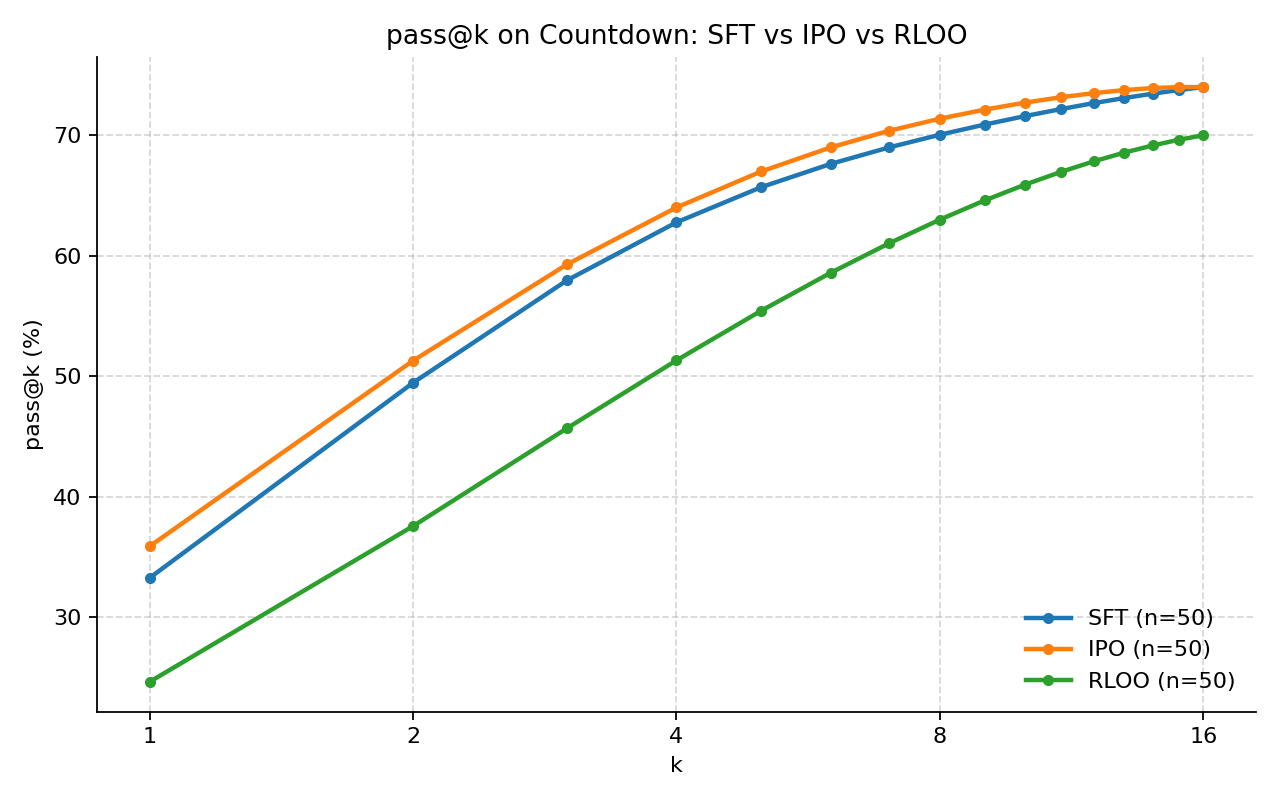
\includegraphics[width=0.7\textwidth]{../passk_comparison.png}
  \caption{Pass@$k$ on the held-out set, SFT versus IPO (RLOO also shown for reference). IPO edges SFT at pass@1 and ties it at pass@16.}
  \label{fig:ipo_pass_k}
\end{figure}

\subsection{Sample Rollout}
A representative IPO rollout on a held-out problem (target 44, numbers 26, 4, 2).
The model tries a few direct combinations, then works backward and lands on
$(26 - 4) \times 2 = 44$. The answer is correct and uses each number once.

\begin{lstlisting}[caption={Sample IPO Test-Set Rollout (Countdown)}, label={lst:ipo_rollout}]
[PROMPT]
Target: 44
Allowed numbers: [26, 4, 2]

[IPO MODEL ROLLOUT]
<think>
Let me analyze this step by step:
1. First, let's try to get close to 44 with basic operations:
- 26 + 2 = 28 (too low)
- 26 + 26 = 52 (too high)
- 4 * 2 = 8 (too low)
2. Let's work backwards from 44:
- 44 is 4 * 11
- So if we could get 11 from the remaining numbers (26, 4), that would work
3. Let's try to get 11:
- 26 - 4 = 22
- 22 - 2 = 20
- Not helpful
4. Another approach:
- 26 - 4 = 22
- 22 * 2 = 44
- And we still have 2 to use
- So if we do (26 - 4) * 2 = 44
This works! Let's verify:
26 - 4 = 22
22 * 2 = 44
</think>
<answer> (26 - 4) * 2 </answer>
\end{lstlisting}

\newpage

\section{RLOO Milestone Component}
\label{sec:rloo_milestone}

\subsection{Training and Evaluation Metrics}
We initialize RLOO from the SFT checkpoint and train for 27 update steps with a
constant learning rate of $1\times10^{-5}$, batch size 128, KL coefficient
$0.001$ to the frozen SFT reference, and an entropy coefficient of $0.001$. For each prompt we
sample a group of $G$ responses and score them with the rule-based verifier. The
Leave-One-Out baseline for a response is the mean reward of the other $G-1$
responses in its group, so the advantage is that response's reward minus the
group mean. Each update applies a sequence-level importance weight to correct for
log-probability mismatch between the vLLM sampler and the trainer.

We use a group size of 8. Mean reward climbed from $0.31$ at step 0 to $0.55$ by
step 27 (Figure~\ref{fig:rloo_reward}) and rollout accuracy rose from $0.24$ to
$0.52$ across the run. The importance weight is clamped to $[0.5, 2.0]$ to bound
the influence of vLLM/HF logprob mismatch on long responses, and gradients are
norm-clipped at $1.0$ so no single update can dominate. Under these safeguards the
weight trends down from $1.78$ to $1.18$ as the policy adapts to the sampler
(Figure~\ref{fig:rloo_importance}), and training remained stable throughout.

\begin{figure}[H]
  \centering
  \begin{minipage}{0.48\textwidth}
    \centering
    
\includegraphics[width=\linewidth]{wandDB-imgs/rloo-train-loss.png}
    \caption{RLOO loss on the train set. Loss climbs smoothly from $\approx -16$ to $\approx 0$ over training.}
    \label{fig:rloo_loss}
  \end{minipage}
  \hfill
  \begin{minipage}{0.48\textwidth}
    \centering
    
\includegraphics[width=\linewidth]{wandDB-imgs/rloo-train-importance-weight.png}
    \caption{Importance weight mean on the train set.}
    \label{fig:rloo_importance}
  \end{minipage}

  \vspace{0.4cm}

  \begin{minipage}{0.48\textwidth}
    \centering
    
\includegraphics[width=\linewidth]{wandDB-imgs/rloo-train-KL-loss.png}
    \caption{KL loss on the train set over training iterations.}
    \label{fig:rloo_kl}
  \end{minipage}
  \hfill
  
  \begin{minipage}{0.48\textwidth}
    \centering
    
\includegraphics[width=\linewidth]{wandDB-imgs/rloo-train-reward-accuracy.png}
    \caption{Rollout accuracy (over 16 samples) on the train set.}
    \label{fig:rloo_accuracy}
  \end{minipage}
\end{figure}

\begin{figure}[H]
  \centering
  
\includegraphics[width=0.48\textwidth]{wandDB-imgs/rloo-train-reward-mean.png}
  \caption{Mean reward on the train set, rising from $0.31$ to $0.55$ over training.}
  \label{fig:rloo_reward}
\end{figure}

\subsubsection{Functional Correctness (Pass@$k$)}
Using the same 50 held-out problems and 16 completions per problem, RLOO reaches
pass@1 $44.8\%$ and pass@16 $68.0\%$, surpassing both SFT ($33.3\%$, $74.0\%$) and
IPO ($35.9\%$, $74.0\%$) at pass@1 by a wide margin. The policy gains roughly 12
percentage points of pass@1 over its SFT starting point; the pass@16 ceiling
decreases slightly as the policy becomes more deterministic, but the gap closes as
$k$ grows. Note: Figure~\ref{fig:rloo_pass_k} below still shows the original RLOO run; we did not have time to regenerate the comparison plot for the fixed checkpoint before the resubmission deadline, but the updated pass@$k$ numbers are reported above.

\begin{figure}[H]
  \centering
  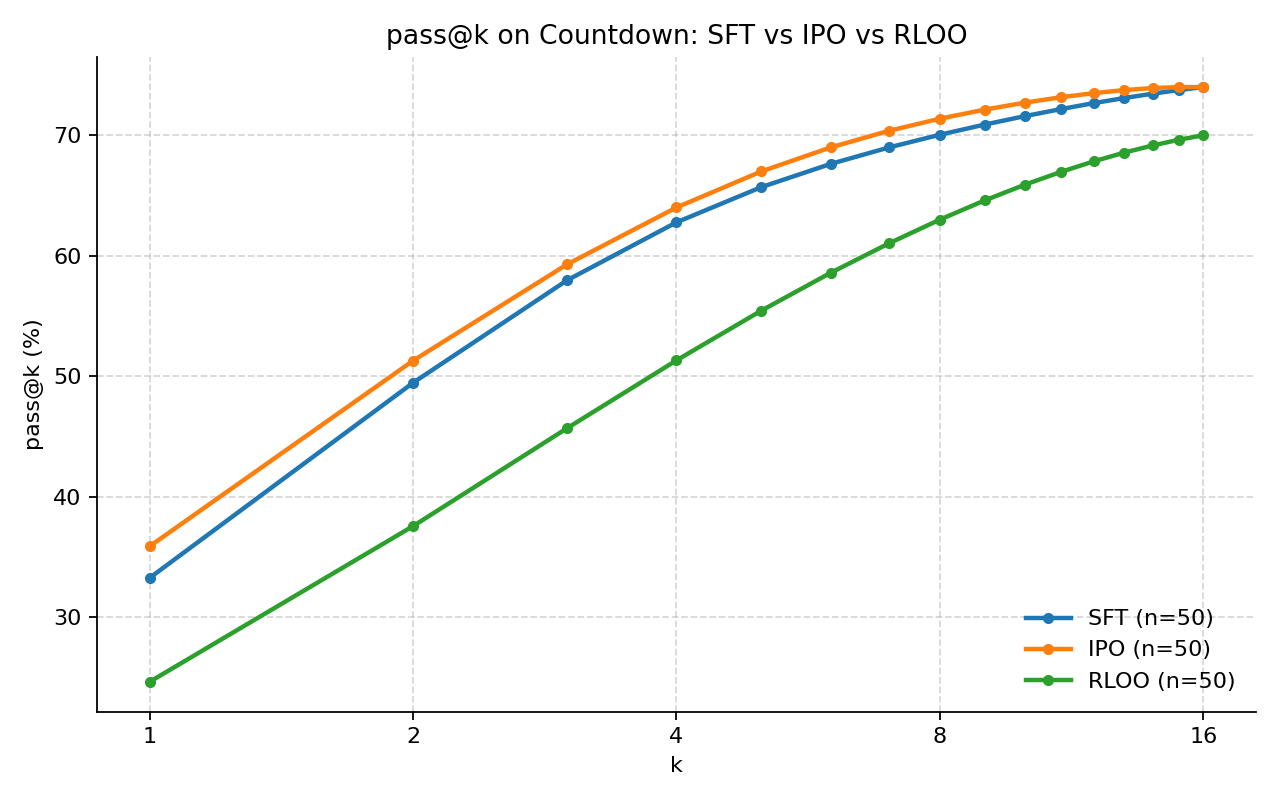
\includegraphics[width=0.7\textwidth]{../passk_comparison.png}
  \caption{Pass@$k$ on the held-out set from the original RLOO run (before the importance-weight clamp and gradient-norm-clip fixes). Updated pass@$k$ values for the fixed checkpoint are reported in the text.}
  \label{fig:rloo_pass_k}
\end{figure}

\subsection{Sample Rollout}
A representative RLOO rollout (target 89, numbers 94, 89, 94). The model notices
the target is one of the given numbers, cancels the two 94s to make 0, and adds
89. Correct, with each number used once.

\begin{lstlisting}[caption={Sample RLOO Test-Set Rollout (Countdown)}, label={lst:rloo_rollout}]
[PROMPT]
Target: 89
Allowed numbers: [94, 89, 94]

[RLOO MODEL ROLLOUT]
<think>
Let me analyze this step by step:
1. Since 89 is one of our numbers and it's also the target, let's see if we can get there directly.
2. We have two 94s and 89 left. Let's see if we can use these to cancel out or equal 89.
3. 94 - 94 = 0, which is close to 89. This could be useful.
4. If we have 0, we can add 89 to get 89.
5. Let's verify: (94 - 94) + 89 = 0 + 89 = 89
6. This works perfectly! We can write this as: 94 - 94 + 89
</think>
<answer>94 - 94 + 89</answer>
\end{lstlisting}

\newpage

\section{Extension Updates (Optional)}
\label{sec:extension_updates}
Describe any progress, modifications, or updates regarding your project extension here. (You may remove or leave this section blank if you do not have updates to report at this stage).

\newpage

\section{Team Contributions}
\label{sec:contributions}
The proposal listed three members, with the default pipeline split evenly across
all three. Nicolo has since dropped the course, so the team for this milestone is
Nick Allen and Finn Staeblein, and we divided the work evenly between us. Nick
owned the IPO component (trainer, training runs, and IPO evaluation) and Finn
owned the RLOO component (update worker, training runs, and RLOO evaluation).
Both members ran the shared SFT and pass@$k$ pipeline and wrote the report
together. For the remaining work on the conjecturer-prover extension, we plan to
keep an even split across the conjecturer-side problem generation and
difficulty-band reward, the prover-side RLOO integration, and the
out-of-distribution evaluation.

\newpage

% References
\bibliographystyle{plainnat}
\bibliography{reference}

\end{document}